% ------------------------------------------------
% LaTeX Template for ML/AI Research Paper
% ------------------------------------------------

\documentclass[11pt]{article}

% ------------------------------------------------
% Packages
% ------------------------------------------------
\usepackage{amsmath, amssymb}
\usepackage{graphicx}
\usepackage{hyperref}
\usepackage{natbib}          % For bibliography
\usepackage{geometry}        % For adjusting margins
\usepackage{times}           % For Times New Roman font
\usepackage{float}           % For controlling float positions
\usepackage{booktabs}        % For professional-looking tables
\usepackage{caption}
\usepackage{subcaption}
\usepackage{color}

% ------------------------------------------------
% Page Setup
% ------------------------------------------------
\geometry{margin=1in}

% ------------------------------------------------
% Title and Author Information
% ------------------------------------------------
\title{Credit Card Fraud Detection using ML Algorithm}
\author{
  Andrew Green\thanks{Corresponding author: \texttt{asong5@uncc.edu}} \\   
  % Add more authors if necessary
}
\date{\today}

% ------------------------------------------------
% Document Begins
% ------------------------------------------------
\begin{document}

\maketitle

% ------------------------------------------------
% Abstract
% ------------------------------------------------
\begin{abstract}
% Provide a concise summary of the entire paper (150-250 words).
% Include background, methods, results, and conclusions.
This study investigates machine learning algorithms for credit card fraud detection
using dataset that contains transactions made by credit cards in September 2013
 by European cardholders. We explore Decision Trees and Deep Learning with Tensor-
Flow, addressing class imbalance with oversampling technique. Our findings reveal
modest performance improvements in Decision tree when oversampling technique 
are applied to the dataset.
\end{abstract}

% Optionally, you can add keywords
% \vspace{0.5cm}
% \noindent\textbf{Keywords:} Keyword1, Keyword2, Keyword3

% ------------------------------------------------
% Main Content
% ------------------------------------------------

% 1. Introduction
\section{Introduction}
In recent years, the rapid growth of online transactions and digital payment platforms has led to a significant increase in credit card fraud. As financial institutions and consumers become more reliant on electronic transactions, the need for robust, accurate, and efficient fraud detection systems has never been greater. Traditional fraud detection methods, which often rely on rule-based systems or manual reviews, struggle to keep up with the evolving tactics of fraudsters and the sheer volume of transactions. 

Machine learning (ML) offers a promising solution to this challenge. By learning patterns from historical transaction data, ML algorithms can identify potentially fraudulent activities with high accuracy and speed, often detecting fraud that may be missed by conventional approaches. This project aims to leverage machine learning techniques to build a credit card fraud detection model capable of distinguishing between legitimate and fraudulent transactions.

In this study, we utilize a real-world credit card transaction dataset containing over 284,000 samples and 30 features. We explore two different machine learning algorithms — a Decision Tree Classifier and a Neural Network — to develop and evaluate models for detecting fraudulent transactions. Additionally, we address the significant class imbalance problem inherent in fraud detection datasets using oversampling techniques to improve model performance.

By the end of this project, we aim to demonstrate the effectiveness of ML models in credit card fraud detection and provide insights into how data preprocessing, algorithm selection, and handling class imbalance can influence the accuracy and reliability of fraud detection systems.

% 2. Methodology
\section{Literature Review}
Credit card fraud detection has been an active area of research due to its critical importance in finance and e-commerce. Over the years, various approaches have been proposed to improve the accuracy and efficiency of fraud detection systems. Traditional methods often relied on rule-based systems, expert knowledge, and statistical techniques such as logistic regression. However, these approaches face challenges in adapting to the dynamic and evolving nature of fraudulent behavior.

Machine learning (ML) has emerged as a powerful alternative, offering the ability to automatically learn complex patterns from large volumes of data. Among the widely used ML algorithms in fraud detection are Decision Trees, Random Forests, Support Vector Machines (SVM), and Neural Networks. Decision Trees provide an interpretable model structure and have been shown to perform well on structured data like transaction records. Neural Networks, particularly deep learning models, excel at capturing nonlinear relationships and interactions among features, although they often require more computational resources and careful tuning.

Several studies have highlighted the benefits of using ML in fraud detection. For instance, Dal Pozzolo et al. (2015) demonstrated the effectiveness of ensemble learning techniques and data resampling methods for handling class imbalance — a common issue where fraudulent transactions represent a tiny fraction of all data. Similarly, Carcillo et al. (2018) explored the use of advanced anomaly detection methods and emphasized the importance of robust evaluation metrics beyond accuracy, such as precision, recall, and the F1-score.

The challenge of imbalanced data is particularly critical. Without addressing this imbalance, ML models tend to be biased towards the majority class (genuine transactions), leading to poor detection of fraudulent cases. Techniques such as oversampling the minority class or using cost-sensitive learning have been proposed and widely adopted in the literature.

In this project, we build upon these established practices by implementing a Decision Tree Classifier and a Neural Network model. We also apply oversampling techniques to mitigate data imbalance, following the recommendations and findings from prior research in the field.

\section{Methods}
In this section, we present a comprehensive overview of the methods and techniques used in our credit card fraud detection. We evaluated the performance of Decision Trees and subsequently assessed their performance on the testing data. For Deep Learning with TensorFlow, we trained the model on the training data and evaluated its performance on the testing data. To tackle the issue of class imbalance, we test the Resampling technique by oversampling the minority class (creating synthetic data) to balance the dataset. Lastly, we applied the Decision Tree and Deep Learning algorithm on the resampled dataset and compare their performance with algorithms without resampling.

\subsection{Decision Trees}
A Decision Tree Algorithm is a supervised machine learning model that uses a tree-like structure to make sequential decisions for classification or regression tasks. It works by recursively splitting data based on features to create branches, with each leaf node representing a predicted outcome.

The tree-like structure starts with one main question at the top called a node which further branches out into different possible outcomes where:

\begin{itemize}
	\item Root Node is the starting point that represents the entire dataset.
	
	\item Branches: These are the lines that connect nodes. It shows the flow from one decision to another.
	
	\item Internal Nodes are Points where decisions are made based on the input features.
	\item Leaf Nodes: These are the terminal nodes at the end of branches that represent final outcomes or predictions
\end{itemize}

For instance, in the example below, decision trees learn from data to approximate a sine curve with a set of if-then-else decision rules. The deeper the tree, the more complex the decision rules and the fitter the model.

\begin{figure}[H]
	\centering
	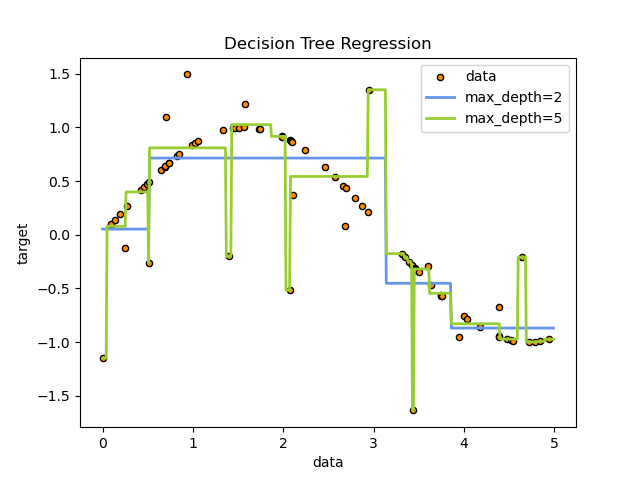
\includegraphics[width=0.7\textwidth]{figure/decision_tree.png}
	\caption{Decision Tree.}
	\label{fig:DecisionTree}
\end{figure}

Some advantages of decision trees are:
\begin{itemize}
	\item Simplicity and Interpretability: Decision trees are straightforward and easy to understand. You can visualize them like a flowchart which makes it simple to see how decisions are made.	
	
	\item Versatility: It means they can be used for different types of tasks can work well for both classification and regression
	
	\item No Need for Feature Scaling: They don’t require you to normalize or scale your data. 
	
	\item Handles Non-linear Relationships: It is capable of capturing non-linear relationships between features and target variables.	
\end{itemize}


The disadvantages of decision trees include:
\begin{itemize}
\item Overfitting: Overfitting occurs when a decision tree captures noise and details in the training data and it perform poorly on new data.

\item  Instability: instability means that the model can be unreliable slight variations in input can lead to significant differences in predictions.

\item Bias towards Features with More Levels: Decision trees can become biased towards features with many categories focusing too much on them during decision-making. This can cause the model to miss out other important features led to less accurate predictions .
\end{itemize}

\subsection{Deep Learning with Tensorflow}
Deep Learning is a powerful technique for building neural network models that can learn complex representations of data. In our study, we utilize Deep Learning with TensorFlow to predict credit risk. TensorFlow is an open-source machine learning platform that provides high-level APIs for building neural networks, as well as low-level APIs for customization and optimization of models. Specifically, we use the Keras API in TensorFlow to construct our neural network model for credit risk assessment.

Our neural network model consists of three fully connected layers, with 128 units in the first and second layers. The input shape of the first layer is determined by the number of features in the input data. We use the rectified linear unit (ReLU) activation function in the first two layers to introduce nonlinearity, and the sigmoid activation function in the output layer to produce a binary classification output. We also include dropout layers after the first and second layers with a rate of 0.2 to prevent overfitting.

During training, the L2 regularization is been used to prevent overfitting by adding a penalty term to the model's loss function. This penalty discourages the model from becoming too complex, which can lead to poor performance on new, unseen data. Essentially, regularization helps the model generalize better by balancing the trade-off between fitting the training data and keeping the model simple.  

We compile the model using the binary cross-entropy loss function and the Adam optimizer.The model is trained on the training data for a maximum of 20 epochs with a batch size of 32. 

The decision function for our Deep Learning model is given by:
\begin{equation}
f(x) = \text{sign}(w^T_3 a_2 + b_3)
\end{equation}

where $w_3$ is the weight vector for the output layer, $a_2$ is the output of the second hidden layer, and $b_3$ is the bias term for the output layer. 

The output of the second hidden layer is given by:

\begin{equation}
a_2 = \text{ReLU}(w^T_2 a_1 + b_2)
\end{equation}

where $w_2$ is the weight matrix for the second hidden layer, $a_1$ is the output of the first hidden layer, and $b_2$ is the bias vector for the second hidden layer. 

The output of the first hidden layer is given by:

\begin{equation}
	a_1 = \text{ReLU}(w^T_1 x + b_1)
\end{equation}

where $w_1$ is the weight matrix for the first hidden layer, $x$ is the input feature vector, and $b_1$ is the bias vector for the first hidden layer.
 
Binary cross-entropy (log loss) is a loss function used in binary classification problems. It quantifies the difference between the actual class labels (0 or 1) and the predicted probabilities output by the model. The lower the binary cross-entropy value, the better the model’s predictions align with the true labels.

Mathematically, Binary Cross-Entropy (BCE) is defined as:

\begin{equation}
	BCE = - \frac{1}{N}\sum_{i=1}^{N}[y_i \log(p_i) + (1- y_i)\log(1-p_i)]	 
\end{equation}	
where
\begin{itemize}
	\item $N$ is the number of observations
	\item $y_i$ is the actual binary label (0 or 1) of the $i^{th}$ observation.
    \item $p_i$ is predicted probability of the $i^{th}$ observation being in class 1.	 
\end{itemize}

Since the model’s output is a probability between 0 and 1, minimizing binary cross-entropy during training helps improve predictive accuracy, ensuring the model effectively distinguishes between two classes.

% 3. Experiments
\section{Data Description and Prerpocessing}
The primary objective of this project is to develop a machine learning-based system capable of accurately detecting fraudulent credit card transactions. We aim to design, implement, and evaluate two different ML algorithms — a Decision Tree Classifier and a Neural Network — using a real-world dataset containing anonymized credit card transactions.

\subsection{Dataset}
The dataset used in this project was obtained from Kaggle's Credit Card Fraud Detection dataset \cite{cc_default}, which contains 284,807 transactions, each described by 30 features. These features include numerical transformations of the original data (denoted V1 through V28) obtained via Principal Component Analysis (PCA) to protect confidentiality. The dataset also includes the transaction amount and a class label indicating whether the transaction is legitimate (0) or fraudulent (1).

The figure \ref{fig:Data Structure} below shows the structure of the dataset where all attributes are shown, with their type, in addition to a glimpse of the variables within each
Attribute.

\begin{figure}[H]
	\centering
	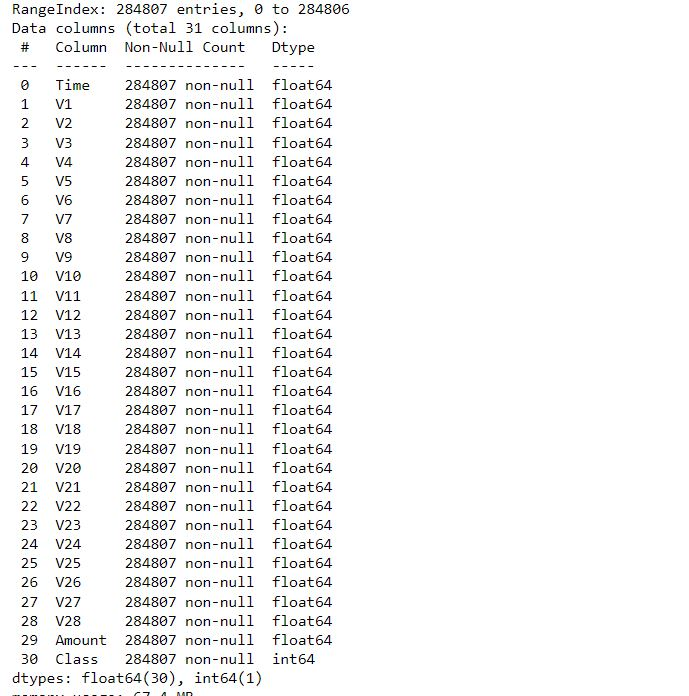
\includegraphics[width=0.8\textwidth]{figure/Data_Structure.jpg}
	\caption{Data Structure}
	\label{fig:Data Structure}
\end{figure} 

Among 284,315 genuine transactions, there are 492  fraudulent transactions, which accounted for only 0.17\% of the data. This extreme imbalance was visualized in figure \ref{fig:Class Count}, confirming the disproportion between classes.

\begin{figure}[H]
	\centering
	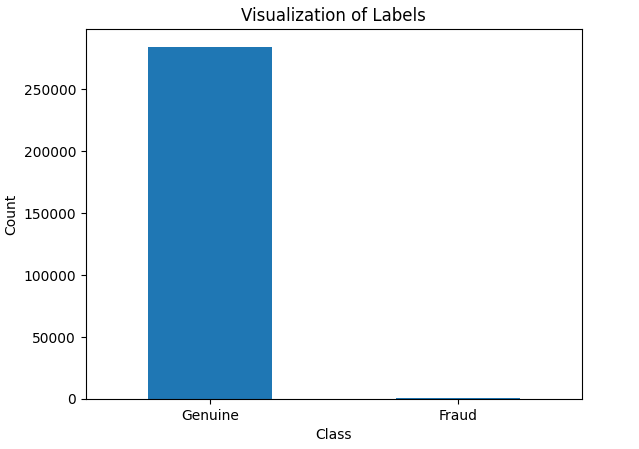
\includegraphics[width=0.8\textwidth]{figure/Count_Class.png}
	\caption{Class Count}
	\label{fig:Class Count}
\end{figure}

% 4. Results
\subsection{Data preprocessing}
% Present the findings of your experiments.
% - Quantitative Results (Use tables and figures)
% - Qualitative Results
% - Comparisons
% - Statistical Analysis

% Example of including a figure
% \begin{figure}[H]
%     \centering
%     \includegraphics[width=0.7\textwidth]{path/to/your/image.png}
%     \caption{Caption of the figure.}
%     \label{fig:label}
% \end{figure}

% Example of including a table
% \begin{table}[H]
%     \centering
%     \caption{Caption of the table.}
%     \label{tab:label}
%     \begin{tabular}{lcc}
%         \toprule
%         Header1 & Header2 & Header3 \\
%         \midrule
%         Row1 & Data & Data \\
%         Row2 & Data & Data \\
%         \bottomrule
%     \end{tabular}
% \end{table}

Before the data was split into train, valid and test data set, the Amount feature was normalized using StandardScaler to ensure that it did not disproportionately influence the models. The "Time" feature was also removed as it was not relevant for fraud detection.

The dataset was then split into training (64\%), validation (16\%), and test (20\%) sets for model development and evaluation.

\subsection{Handling Class Imbalance}

To address the imbalance problem, we applied Random Oversampling to the training data, creating synthetic instances of fraudulent transactions to balance the classes. 

This step ensured that the models received balanced data during training, improving their ability to detect fraud effectively.

% 5. Discussion
\section{Algorithm and performance analysis}
% Interpret the results and discuss their implications.
% - Insights
% - Limitations
% - Practical Implications
% - Theoretical Implications
This project utilized two different machine learning algorithms for credit card fraud detection: a Decision Tree Classifier and a Neural Network. Both models were evaluated on the original imbalanced dataset and on the oversampled balanced dataset to assess the impact of class imbalance.

\subsection{Decision Tree Algorithm}
 
A Decision Tree Classifier was trained on the original dataset without any class balancing. The model achieved the following performance on the test set:

\begin{table}[H]
  \centering
  \caption{Decision Tree Results}
  \label{tab:decision_tree}
  \begin{tabular}{lcc}
       \toprule
       Metric & Value \\
       \midrule
       Accuracy &  99.916\% \\
       Precision &  74.51\% \\
       Recall &  77.55\%  \\
       F1-score &  75.38\% \\              
       \bottomrule
 \end{tabular}
\end{table} 

The confusion matrix for Decision Tree is in figure \ref{fig:confusion_matrix}

\begin{figure}[H]
	\centering
	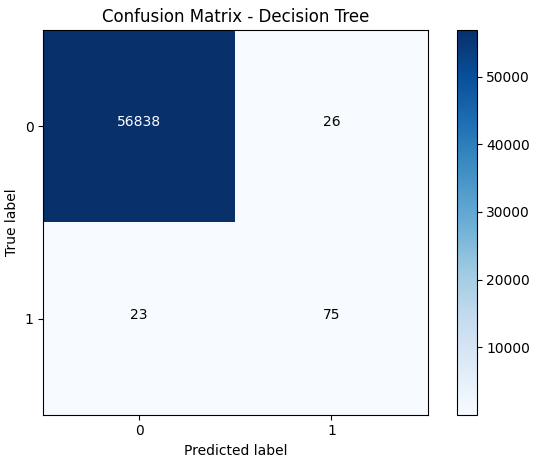
\includegraphics[width=0.8\textwidth]{figure/confusion_matrix.png}
	\caption{Data Structure}
	\label{fig:confusion_matrix}
\end{figure} 

While the overall accuracy was very high, the relatively lower precision and recall indicated that the model struggled to identify fraudulent transactions effectively due to the severe class imbalance.

\subsection{Decision Tree Algorithm with resampled Data}
After a Decision Tree Classifier was trained again over the resampled data, the model achieved the following performance on the test data set:

\begin{table}[H]
	\centering
	\caption{Decision Tree Results with resampled data}
	\label{tab:decision_tree resample}
	\begin{tabular}{lcc}
		\toprule
		Metric & Value \\
		\midrule
		Accuracy &  99.97\% \\
		Precision &  99.94\% \\
		Recall &  1.00\%  \\
		F1-score &  99.97\% \\              
		\bottomrule
	\end{tabular}
\end{table} 

The confusion matrix for Decision Tree is in figure \ref{fig:confusion_matrix_resample}

\begin{figure}[H]
	\centering
	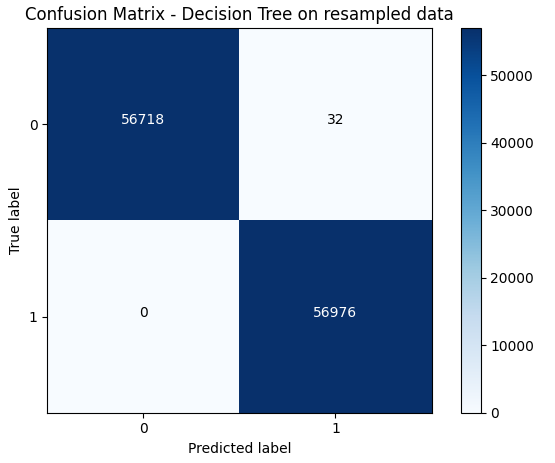
\includegraphics[width=0.8\textwidth]{figure/confusion_matrix_resample.png}
	\caption{Data Structure}
	\label{fig:confusion_matrix_resample}
\end{figure} 

The improvement in precision and recall demonstrated that oversampling helped the model better distinguish fraudulent transactions.

\subsection{Neural Network Algorithm}

Original (Imbalanced) Data
A Neural Network with two hidden layers (each containing 128 neurons with ReLU activation and L2 regularization) was implemented using Keras. The visual model structure is in Figure \ref{fig:model_structure}: 

\begin{figure}[H]
	\centering
	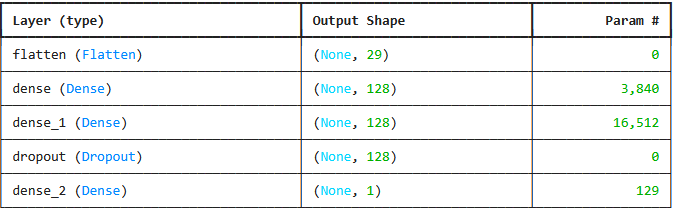
\includegraphics[width=0.8\textwidth]{figure/model_structure.png}
	\caption{Model Structure}
	\label{fig:model_structure}
\end{figure} 

After model fitting on training data, the model achieved:
 Test Accuracy: 99.92\%

However, like the Decision Tree, the neural network’s recall and precision were limited due to the class imbalance, though accuracy remained high.

\subsection{Neural Network Algorithm with resampled data}
Oversampled (Balanced) Data
The Neural Network was retrained on the oversampled data:

Test Accuracy: 99.52%

While the accuracy slightly decreased after balancing, this was expected due to the introduction of synthetic minority class samples. However, the model’s ability to detect fraud improved significantly when precision and recall were considered. 

% 6. Conclusion
\section{Conclusion}
% Summarize the research and suggest future directions.
% - Summary of findings
% - Significance
% - Future Work
This project successfully demonstrated the application of machine learning algorithms for credit card fraud detection using a real-world dataset. Two models — a Decision Tree Classifier and a Neural Network — were developed and evaluated on both the original imbalanced data and a balanced dataset created through Random Oversampling. 

Both models initially showed excellent accuracy but suffered from poor fraud detection performance because of the imbalance between genuine and fraudulent transactions. Oversampling successfully mitigated this issue.

Key findings from the project include:

\begin{itemize}
	\item Both models achieved high accuracy on the imbalanced dataset, but their ability to detect fraudulent transactions (as measured by precision and recall) was limited due to the severe class imbalance. 
	
	\item After applying oversampling, the Decision Tree achieved near-perfect performance, with a recall of 100\% and an F1-score of 99.969\%. This demonstrated the model’s improved ability to correctly identify fraudulent transactions.
	
	\item The Neural Network also showed improved fraud detection capability after balancing the data, though with a slight decrease in overall accuracy — an expected trade-off when improving minority class detection.	
\end{itemize}	

Throughout the project, it became evident that handling data imbalance is crucial for the success of fraud detection models. Without addressing this issue, models tend to perform poorly in identifying the minority class, which, in this case, represents the critical fraud cases. 

Overall, this project demonstrated the potential and effectiveness of machine learning approaches in fraud detection and underscored the importance of thoughtful data handling and evaluation strategies.
 

% 8. Acknowledgments
\section*{Acknowledgments}
% Credit those who contributed to the research but are not listed as authors.
% - Funding Sources
% - Collaborations

% ------------------------------------------------
% References
% ------------------------------------------------
\bibliographystyle{plainnat}
\bibliography{references}

% ------------------------------------------------
% Appendices (Optional)
% ------------------------------------------------
\appendix


% ------------------------------------------------
% Document Ends
% ------------------------------------------------
\end{document}
